\documentclass[11pt,a4paper]{article}
\usepackage[top=3cm, bottom=2cm, left=2cm, right=2cm]{geometry}
\usepackage[utf8]{inputenc}
% \usepackage[T1]{fontenc}
\usepackage{amsmath, amsfonts, amssymb}
\usepackage{siunitx}
\usepackage[brazil]{babel}
\usepackage{graphicx}
\usepackage[margin=10pt,font={small, it},labelfont=bf, textfont=it]{caption}
\usepackage[dvipsnames, svgnames]{xcolor}
\DeclareCaptionFont{MediumOrchid}{\color[svgnames]{MediumOrchid}}
\usepackage[pdftex]{hyperref}
\usepackage{natbib}
\bibliographystyle{plainnat}
\bibpunct{[}{]}{,}{s}{}{}
\usepackage{color}
\usepackage{footnote}
\usepackage{setspace}
\usepackage{booktabs}
\usepackage{multirow}
\usepackage{subfigure}
\usepackage{fancyhdr}
\usepackage{leading}
\usepackage{indentfirst}
\usepackage{wrapfig}
\usepackage{mdframed}
\usepackage{etoolbox}
\usepackage[version=4]{mhchem}
\usepackage{enumitem}
\usepackage{caption}
\usepackage{titlesec}
\usepackage{tcolorbox}
\usepackage{tikz}
\usepackage{LobsterTwo}
\usepackage[T1]{fontenc}
\usepackage{fontspec}
\usepackage{txfonts}
\AtBeginEnvironment{equation}{\fontsize{13}{16}\selectfont}


\titleformat{\section}{\LobsterTwo\LARGE\color{CarnationPink}}{\thesection.}{1em}{}
\titleformat{\subsection}{\LobsterTwo\LARGE\color{CarnationPink}}{\thesubsection}{1em}{}


\DeclareCaptionLabelFormat{figuras}{\textcolor{DarkTurquoise}{Figura \arabic{figure}}}
\captionsetup[figure]{labelformat=figuras}

\makeatletter
\renewcommand\tagform@[1]{\maketag@@@{\color{CarnationPink}(#1)}}
\makeatother

\renewcommand{\theequation}{Eq. \arabic{equation}}
\renewcommand{\thefigure}{Fig. \arabic{figure}}
\renewcommand{\thesection}{\textcolor{CarnationPink}{\arabic{section}}}

\setlist[itemize]{label=\textcolor{CarnationPink}{$\mathbf{\square}$}}

\setlist[enumerate]{label=\textcolor{CarnationPink}{\arabic*.}, align=left}


\newcounter{exemplo}

\NewDocumentEnvironment{exemplo}{ O{} }{%
\allowbreak
\setlength{\parindent}{0pt}
  \begin{mdframed}[
  leftline=true,
  topline=false,
  rightline=false,
  bottomline=false,
  linewidth=2pt,
  linecolor=CarnationPink,
  frametitlerule=false,
  frametitlefont=\LobsterTwo\large\color{CarnationPink},
  frametitle={\color{CarnationPink}\LobsterTwo\large #1},
  ]
}{%
  \end{mdframed}
}

\setlength{\fboxsep}{5pt}
\setlength{\fboxrule}{1.5pt}
\usepackage{float}
\renewcommand{\thefootnote}{\alph{footnote}}
\usepackage{url}
\hypersetup{
	colorlinks=true,
	linkcolor=DarkTurquoise,
	filecolor=DarkTurquoise,      
	urlcolor=DarkTurquoise,
	citecolor=DarkTurquoise,
	pdftitle={Radioterapia}
}
\pagestyle{fancy}
\fancyhf{}
\renewcommand{\headrulewidth}{0pt}
\rfoot{Página \thepage}

\title{\LobsterTwo\Huge{Radiobiologia}}
\author{\LobsterTwo{Biologia Molecular\nocite{*}}}
\date{\LobsterTwo\textit{Dalila Mendonça}}
\begin{document}
	\maketitle

	\section{Introdução}

		O alvo da radiação para fins terapêuticos é o DNA. O DNA é composto de açúcares, fosfatos e bases e formará superestruturas com outras proteínas para formar cromossomos, que podem ser vistos ao microscópio na fase M. Dentro do cromossomo estão os genes que podem ser transcritos em proteínas. A função desses genes pode ser alterada por mutações ou por mudanças epigenéticas em expressão. A expressão de genes de RNA pode ser visualizada e medida por meio de perfis de matriz de expressão gênica, agrupamento hierárquico, RT-PCR quantitativo e RNAseq de célula única. Os níveis de RNA podem ser regulados por transcrição e microRNAs. Uma vez traduzidas, as células podem regular a atividade da proteína por: translocação; modificações como fosforilação e metilação; e degradação pelo ``proteasome'' após a ``ubiquitination''. Verificou-se que a sinalização nas células está ligada a várias vias de transdução de sinal cujas proteínas regulam o crescimento celular, o controle do ciclo celular, a divisão celular e a morte celular. Essas proteínas podem ser receptores de superfície celular, ligantes que se ligam a receptores de superfície celular, proteínas intermediárias de sinalização e ativadores como fatores de transcrição, proteínas apoptóticas como proteínas BCL2 ou BAX. A radiação pode causar vários tipos diferentes de morte celular, que se combinam com vários mediadores e vias para exibir os efeitos agudos e tardios clinicamente evidentes da radiação.
  
    \section{DNA}

	    O DNA é o principal alvo da radiação, onde a informação vai do DNA  (genes) para o RNA (transcrição) para as proteínas (produto genético). O DNA (ácido desoxirribonucleico) é uma molécula complexa que carrega informações genéticas em todos os organismos vivos. É composto por uma sequência específica de nucleotídeos, que são unidades básicas de construção do DNA. Cada nucleotídeo é composto por três componentes principais: um grupo fosfato, um açúcar chamado desoxirribose e uma base nitrogenada.

	    As bases nitrogenadas são responsáveis por fornecer a informação genética no DNA. Existem quatro tipos de bases nitrogenadas presentes no DNA: adenina (A), timina (T), citosina (C) e guanina (G). A adenina se liga à timina, e a citosina se liga à guanina, formando pares complementares de bases.

		\begin{wrapfigure}{l}{0.5\textwidth}
			\centering
			\fcolorbox{DarkTurquoise}{white}{%
				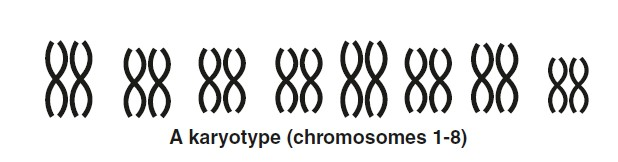
\includegraphics[width=0.45\textwidth]{Imagens/karyotype.jpg}
			}%
			\caption{DNA em um cariótipo parcial}
			\label{fig:karyotype}
		\end{wrapfigure}

	    Essas bases nitrogenadas se unem entre si através de ligações químicas chamadas de pontes de hidrogênio. A adenina forma duas pontes de hidrogênio com a timina, enquanto a citosina forma três pontes de hidrogênio com a guanina. Essas ligações de hidrogênio mantêm as duas cadeias de DNA unidas em uma estrutura de dupla hélice.

	    A dupla hélice é formada pelas duas cadeias de nucleotídeos que se enrolam uma em torno da outra em uma estrutura em forma de espiral. As bases nitrogenadas estão empilhadas no interior da dupla hélice, enquanto os grupos fosfato e açúcar estão na parte externa, formando a chamada "espinha dorsal" do DNA.

		\begin{wrapfigure}{r}{0.35\textwidth}
			\fcolorbox{DarkTurquoise}{white}{%
				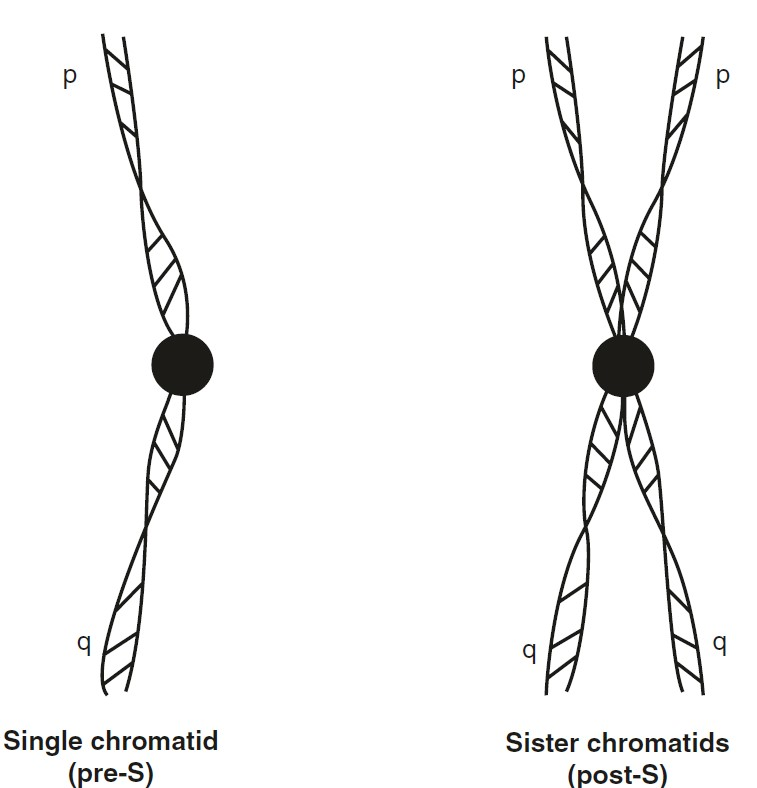
\includegraphics[width=0.3\textwidth]{Imagens/cromatides.jpg}
			}%
			\caption{Cromátide e Cromátides Irmãs}
			\label{fig:cromatides}
		\end{wrapfigure}
	
		
	    As cadeias de DNA são antiparalelas, o que significa que elas estão orientadas em direções opostas. Enquanto uma cadeia é lida de 5' para 3' (cinco prime para três prime), a outra cadeia é lida de 3' para 5'. Essa orientação é importante para a replicação e transcrição do DNA.

	    Além da estrutura em dupla hélice, o DNA pode apresentar diferentes níveis de organização. Os nucleotídeos se organizam em unidades repetitivas chamadas de genes, que contêm as instruções para a síntese de proteínas específicas. Os genes estão localizados em cromossomos, estruturas compostas por DNA e proteínas.

	    Os cromossomos são encontrados no núcleo das células e são responsáveis por armazenar e transmitir as informações genéticas de uma geração para a próxima. Nos seres humanos, cada célula normalmente contém 46 cromossomos, divididos em 23 pares.

	    Em resumo, o DNA é formado por nucleotídeos compostos por um grupo fosfato, um açúcar desoxirribose e uma base nitrogenada (adenina, timina, citosina ou guanina). As bases nitrogenadas se unem através de pontes de hidrogênio, formando uma estrutura em dupla hélice. Os genes estão localizados no DNA e os cromossomos contêm o DNA e proteínas, responsáveis por armazenar e transmitir informações genéticas.

	    A cromatina, cromátide, cromátides irmãs, cromossomo e DNA estão relacionados na organização e estrutura do material genético em uma célula, onde:

    \begin{itemize}
		\item \textcolor{DarkTurquoise}{\textbf{Cromatina: }} A cromatina é a forma de organização do DNA e das proteínas associadas a ele no núcleo das células. A cromatina consiste em filamentos de DNA enrolados em torno de proteínas chamadas histonas. A cromatina permite que o DNA seja compactado e organizado dentro do núcleo celular, ocupando menos espaço.
		\item \textcolor{DarkTurquoise}{\textbf{Cromátide: }} Durante o processo de replicação do DNA, uma molécula de DNA duplica-se para formar duas moléculas idênticas, conhecidas como cromátides. Cada cromátide é uma cópia exata do DNA original e é conectada à sua cromátide irmã por uma região especializada chamada centrômero.
		\item \textcolor{DarkTurquoise}{\textbf{Cromátides irmãs:}} As cromátides irmãs são as duas cópias idênticas de uma molécula de DNA resultantes da replicação do DNA. Elas são mantidas juntas pelo centrômero e estão intimamente ligadas ao longo de sua extensão. Durante a divisão celular, as cromátides irmãs se separam e são distribuídas para cada célula filha.
		\item \textcolor{DarkTurquoise}{\textbf{Cromossomo:}} Um cromossomo é uma estrutura altamente organizada composta por uma única molécula de DNA, que inclui suas cromátides irmãs, e proteínas associadas. Durante a divisão celular, as cromátides irmãs condensam-se e se enrolam ainda mais para formar estruturas compactas visíveis ao microscópio, chamadas de cromossomos. Os cromossomos são responsáveis por manter e transmitir a informação genética de uma célula para outra durante a divisão celular.
		\item \textcolor{DarkTurquoise}{\textbf{DNA:}} O DNA é a molécula que contém as instruções genéticas em um organismo. Ele está presente nas cromátides, que são duplicadas para formar as cromátides irmãs durante a replicação do DNA. O DNA é a base da informação genética e está organizado em genes localizados nos cromossomos. A estrutura em dupla hélice do DNA permite que as informações genéticas sejam copiadas e transmitidas de uma geração para a próxima.
	\end{itemize}

		
		A \ref{fig:cromatides} mostra que um cromossomo pode ser formado por 1 cromátide (pré fase S) ou 2 cromátides irmãs (pós fase s). Porém o DNA é sempre formado por fita dupla, como mostra a \ref{fig:karyotype}, onde mostra um DNA em um cariótipo (parcial). A maioria das células do nosso corpo não está na fase M e não possui cromossomos condensados visíveis. \textit{\textcolor{MediumOrchid}{Um cariótipo é uma representação visual dos cromossomos presentes em uma célula de um organismo, organizados em pares de acordo com seu tamanho, forma e bandas características. É uma forma de analisar e identificar alterações cromossômicas, como anormalidades numéricas (como trissomia do cromossomo 21, responsável pela síndrome de Down) ou anormalidades estruturais (como deleções, duplicações ou translocações).}} 
    
  
    	Como mostra a \ref{fig:cromatides}, Cromossomos não replicados (Pré-S) existem como cromátides p e q, sem cromátides irmãs. Como os humanos são diploides, existem dois de cada cromossomos e os dois cromossomos 4 são diferentes de uns aos outros:, um proveniente do pai e outro da mãe. 

    	Cromossomos replicados (Pos-S) existem como cromátides irmãs idênticas, unidas por um centrômero. Ainda existirá um cromossomo 4 materno e um 4 paterno, mas cada um tem 2 p-arms e 2 q-arms. É normal ver cromossomos apenas replicados porque apenas os cromossomos da fase M são visíveis em um cariótipo tradicional (através do processo de microscopia de luz).

	\section{Replicação do DNA}

	A replicação do DNA é o processo pelo qual uma molécula de DNA é duplicada, resultando em duas moléculas idênticas de DNA. Esse processo é essencial para a transmissão precisa da informação genética de uma célula mãe para suas células filhas durante a divisão celular.

	A replicação do DNA se dá através dos seguintes passos:

	\begin{enumerate}
		\item A molécula de DNA dupla hélice é desenrolada e separada em duas fitas individuais. Isso é feito pela ação da enzima helicase, que quebra as pontes de hidrogênio entre as bases nitrogenadas, desfazendo a estrutura em hélice.
		\item Após o desenrolamento, as fitas de DNA são estabilizadas por proteínas de ligação ao DNA, como as proteínas SSB (single-strand binding proteins). Essas proteínas evitam que as fitas se recombinem novamente.
		\item A enzima primase sintetiza pequenos segmentos de RNA chamados de primers. Os primers fornecem um ponto de partida para a síntese do novo DNA.
		\item A enzima DNA polimerase adiciona os nucleotídeos complementares a cada uma das fitas de DNA em crescimento. A síntese ocorre no sentido 5' para 3', ou seja, a DNA polimerase adiciona novos nucleotídeos à extremidade 3' da fita em crescimento. Em uma fita, chamada de fita líder, a síntese ocorre de forma contínua, enquanto na outra fita, chamada de fita atrasada ou descontínua, a síntese ocorre de forma fragmentada em pequenos segmentos chamados de fragmentos de Okazaki.
		\item A enzima ligase atua unindo os fragmentos de Okazaki, juntando os trechos de DNA descontínuos e formando uma fita contínua.
		\item Durante o processo de replicação, há mecanismos de verificação e correção de erros. A DNA polimerase possui uma atividade de correção de prova, que remove e substitui os nucleotídeos errados. Além disso, outras enzimas, como a exonuclease, também atuam na correção de erros.
		\item Ao final da replicação, existem duas moléculas de DNA idênticas, cada uma composta por uma fita original e uma fita recém-sintetizada.
	\end{enumerate}

	\section{Ciclo Celular}

	O ciclo celular é o processo ordenado e sequencial que ocorre nas células eucarióticas, resultando na duplicação do material genético e na divisão celular em duas células filhas. O ciclo celular é composto por várias fases distintas, cada uma com características específicas e processos envolvidos. A \ref{fig:cicloCelular} apresenta as etapas de um ciclo celular que é dividido em interfase (fases G0, G1, S e G2) e mitose.

	\begin{figure}[h]
		\centering
		\fcolorbox{DarkTurquoise}{white}{%
			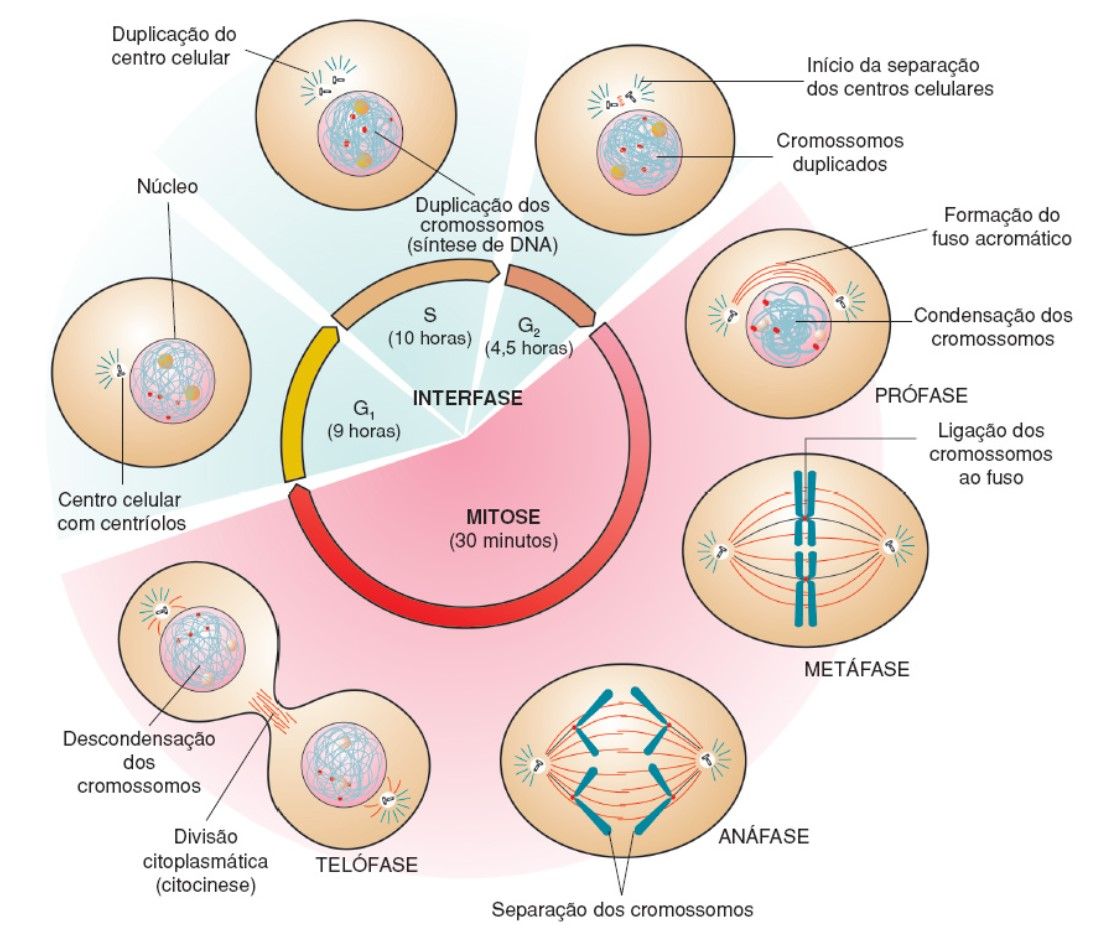
\includegraphics[width=0.52\textwidth]{Imagens/ciclocelular2.jpg}
		}%
	\end{figure}
	\begin{figure}[h]
		\centering
		\fcolorbox{DarkTurquoise}{white}{%
			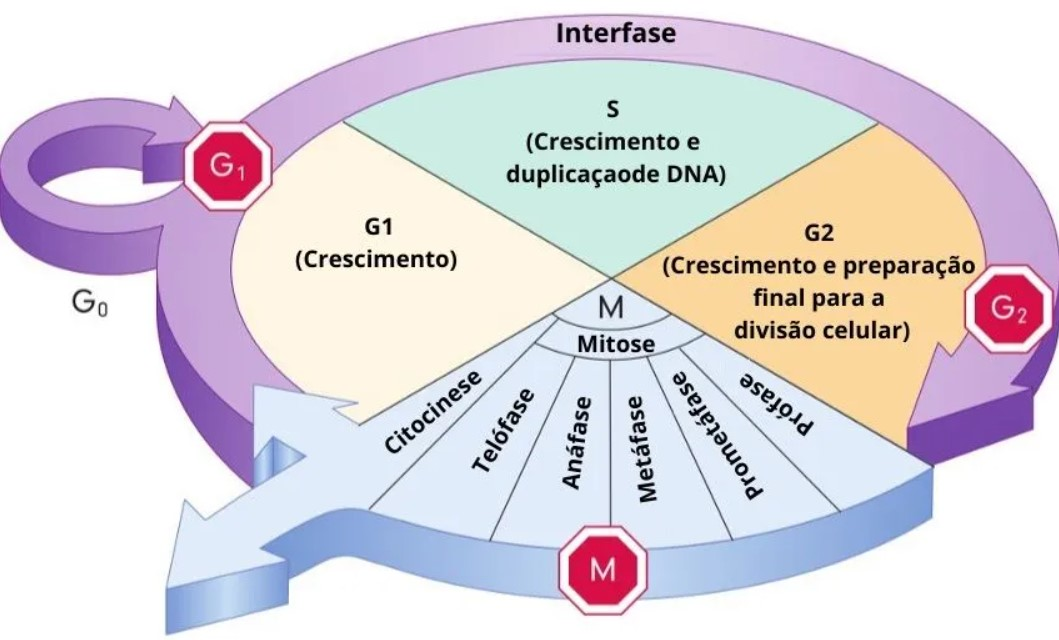
\includegraphics[width=0.52\textwidth]{Imagens/cicloCelularGrande.jpg}
		}%
		\caption{Ciclo Celular}
		\label{fig:cicloCelular}
	\end{figure}
	
	\subsection{Fase G1}

	A fase G1 (Gap 1) é conhecida como fase de crescimento celular. Os principais eventos processos que ocorrem na fase G1 são:

	\begin{enumerate}
		\item \textcolor{DarkTurquoise}{\textbf{Crescimento celular:}} Durante a fase G1, a célula aumenta seu tamanho por meio de síntese de proteínas e aumento do volume citoplasmático. Essa fase acumula os recursos necessários para a próxima fase do ciclo (fase S).
		\item \textcolor{DarkTurquoise}{\textbf{Síntese de proteínas:}} A célula sintetiza proteínas específicas que são necessárias para a replicação do DNA e a divisão celular subsequente. Essas proteínas estão envolvidas na regulação do ciclo celular, na replicação do DNA, na estrutura do citoesqueleto e em outras funções celulares essenciais. Uma das principais proteínas sintetizadas nessa fase são as Ciclinas D. As ciclinas D são proteínas que se ligam a quinases dependentes de ciclina (CDKs) para formar complexos ativos. Elas regulam a transição da fase G1 para a fase S, ativando as CDKs associadas.
		\item \textcolor{DarkTurquoise}{\textbf{Verificação de condições externas:}} Durante a fase G1, a célula verifica se as condições externas e os sinais ambientais são favoráveis para a progressão para a fase S. Se as condições não forem adequadas, a célula pode entrar em um estado não proliferativo chamado G0, onde pode permanecer metabolicamente ativa, mas não está se preparando para se dividir.
		\item \textcolor{DarkTurquoise}{\textbf{Verificação de estado do DNA:}}  Nesta fase, ocorre a verificação da integridade do DNA antes da replicação. A célula verifica se há danos no DNA e se a replicação anterior foi concluída corretamente. Os checkpoints do ciclo celular monitoram a integridade do DNA e impedem que a célula prossiga para a fase S se houver danos ou mutações significativas.
		\item \textcolor{DarkTurquoise}{\textbf{Resposta a sinais de crescimento:}} A célula também responde a sinais de crescimento e fatores de crescimento provenientes do ambiente ou de células vizinhas. Esses sinais podem estimular a entrada da célula na fase S ou desencadear respostas específicas, como diferenciação celular ou apoptose.
	\end{enumerate}

	\subsection{Fase G0}

	A fase G0 (Gap 0) do ciclo celular é um estado quiescente ou não proliferativo em que as células entram quando não estão se preparando para se dividir ou quando interrompem temporariamente seu ciclo de divisão celular. Nessa fase, as células permanecem metabolicamente ativas, mas não passam pelas etapas do ciclo celular para se dividir.

	A fase G0 pode ser um estado transitório ou permanente, dependendo do tipo de célula e do contexto em que se encontra. Algumas células entram em G0 temporariamente, aguardando sinais específicos para reiniciar a divisão celular. Outras células podem entrar em G0 de forma permanente, o que significa que não voltarão a se dividir, como é o caso das células nervosas maduras.

	A fase G0 é importante para permitir que as células desempenhem funções especializadas e executem atividades específicas em tecidos e órgãos. Por exemplo, células musculares, neurônios e células hepáticas maduras geralmente estão em estado G0 para cumprir suas funções especializadas sem a necessidade de se dividir.

	
	\subsection{Fase S}

	Na fase S (síntese de DNA), ocorre a replicação do DNA. Durante essa fase, o material genético presente no núcleo da célula é duplicado, preparando-se para ser distribuído entre as células filhas durante a divisão celular. Os principais eventos processos que ocorrem na fase S são:

	\begin{enumerate}
		\item \textcolor{DarkTurquoise}{\textbf{Replicação do DNA:}} O principal processo que ocorre na fase S é a síntese de uma cópia exata do material genético. Cada cromossomo é replicado, resultando na formação de duas cromátides irmãs. A replicação do DNA é iniciada nos locais específicos chamados origens de replicação, onde as enzimas envolvidas no processo se ligam e iniciam a síntese das novas fitas de DNA. 
		\item \textcolor{DarkTurquoise}{\textbf{Formação de complexos de replicação:}} Durante a fase S, os complexos de replicação são formados nas origens de replicação. Esses complexos são compostos por várias proteínas, incluindo a DNA polimerase, que é a enzima responsável pela síntese das novas fitas de DNA. Múltiplos complexos de replicação são formados simultaneamente ao longo dos cromossomos, permitindo a replicação rápida e eficiente.
		\item \textcolor{DarkTurquoise}{\textbf{Alongamento das fitas de DNA:}} A DNA polimerase adiciona novos nucleotídeos às fitas de DNA existentes, seguindo a complementaridade das bases. As fitas de DNA são desenroladas e as enzimas envolvidas no processo de replicação movem-se ao longo do DNA, adicionando nucleotídeos complementares a cada uma das fitas. Dessa forma, são sintetizadas duas fitas complementares para cada fita de DNA original.
		\item \textcolor{DarkTurquoise}{\textbf{Verificação da fidelidade da replicação:}}  Durante a síntese do DNA, ocorrem mecanismos de verificação e correção de erros para garantir a fidelidade da replicação. Enzimas especializadas verificam a correspondência correta das bases nucleotídicas e corrigem qualquer erro que possa ocorrer durante o processo. Isso é importante para manter a integridade do material genético.
	\end{enumerate}

	Após a conclusão da fase S, cada cromossomo é composto por duas cromátides irmãs, idênticas entre si e ao cromossomo original. Essas cromátides permanecem unidas pelo centrômero, pronto para serem separadas durante a fase M do ciclo celular, conhecida como mitose. A replicação do DNA é um processo altamente regulado e ocorre de maneira precisa para garantir a transmissão correta do material genético para as células filhas.

	\subsection{Fase G2}

	Na fase G2 (Gap 2), ocorrem diversos processos que preparam a célula para a entrada na fase de divisão celular, a fase M (mitose). A fase G2 é uma etapa crítica para garantir que a célula esteja pronta para se dividir de forma correta e eficiente. Os principais eventos processos que ocorrem na fase G2 são:

	\begin{enumerate}
		\item \textcolor{DarkTurquoise}{\textbf{Síntese de proteínas e crescimento:}} Durante a fase G2, a célula continua a sintetizar proteínas e a crescer. O objetivo é acumular recursos celulares e energia para apoiar a divisão celular iminente. Proteínas envolvidas na regulação do ciclo celular, na formação do citoesqueleto e em outras funções essenciais são sintetizadas. Uma das principais proteínas sintetizadas nessa fases são as Ciclinas A. As ciclinas A são proteínas que se ligam a CDKs para formar complexos ativos. Elas regulam a transição da fase G2 para a fase M, preparando a célula para a divisão celular.
		\item \textcolor{DarkTurquoise}{\textbf{Verificação do DNA replicado:}} Nessa fase, a célula verifica se a replicação do DNA ocorreu corretamente durante a fase S. Enzimas de reparo de DNA examinam o material genético para identificar e corrigir possíveis erros e danos no DNA. A célula precisa garantir que o DNA esteja íntegro e sem mutações antes de prosseguir para a fase M.
		\item \textcolor{DarkTurquoise}{\textbf{Verificação de checkpoints do ciclo celular:}} xistem checkpoints do ciclo celular na fase G2 que monitoram se as condições são adequadas para a divisão celular prosseguir. Esses checkpoints avaliam a integridade do DNA, a ocorrência correta da replicação do DNA e a sinalização adequada das fases anteriores do ciclo celular. Se ocorrerem erros ou anormalidades, a célula pode ser levada a interromper o ciclo celular ou a realizar reparos antes de prosseguir para a fase M.
		\item \textcolor{DarkTurquoise}{\textbf{Preparação para a mitose:}} Durante a fase G2, a célula também se prepara para a fase de divisão celular propriamente dita, a mitose. Isso envolve a organização e montagem do fuso mitótico, uma estrutura de microtúbulos que ajudará na separação correta dos cromossomos durante a mitose. Os centrossomos, estruturas celulares importantes para a formação do fuso mitótico, também se replicam nessa fase.
		\item \textcolor{DarkTurquoise}{\textbf{Regulação do ciclo celular:}} Vários sinais e proteínas reguladoras do ciclo celular são ativados e desativados durante a fase G2 para garantir a coordenação adequada das diferentes fases do ciclo. Complexos de proteínas, como as ciclinas e as quinases dependentes de ciclina, são responsáveis por controlar a progressão do ciclo celular e garantir que cada fase ocorra no momento adequado.
	\end{enumerate}

	A fase G2 desempenha um papel crítico na verificação final do DNA, na preparação do aparato mitótico e na regulação do ciclo celular, garantindo uma divisão celular correta e bem coordenada.

	\subsection{Fase M}

	A fase M (Mitose) do ciclo celular é a fase em que ocorre a divisão celular propriamente dita. É subdividida em várias etapas: prófase, prometáfase, metáfase, anáfase e telófase. Durante a fase M, o material genético é segregado de maneira equitativa entre as células filhas. Os principais eventos e processos que ocorrem na fase M são:

	\begin{enumerate}
		\item \textcolor{DarkTurquoise}{\textbf{Prófase:}} é a primeira etapa da fase M e é caracterizada por grandes mudanças na célula. Nesta etapa os cromossomos condensam-se, tornando-se mais curtos e espessos. O envelope nuclear desintegra-se, liberando os cromossomos no citoplasma. Os centríolos começam a se mover para os polos opostos da célula, e o fuso mitótico começa a se formar;
		\item \textcolor{DarkTurquoise}{\textbf{Prometáfase:}} nesta etapa os cromossomos tornam-se ainda mais condensados e visíveis sob o microscópio. Os microtúbulos do fuso mitótico se ligam aos cinetócoros, que são estruturas proteicas localizadas nos centrômeros dos cromossomos. Isso permite que os cromossomos se movam ativamente dentro da célula;
		\item \textcolor{DarkTurquoise}{\textbf{Metáfase:}} os cromossomos se alinham em uma região específica chamada placa equatorial ou placa metafásica. Os microtúbulos do fuso mitótico exercem tensão sobre os cinetócoros dos cromossomos, mantendo-os alinhados corretamente no centro da célula. Esse alinhamento é crucial para garantir a segregação correta do material genético nas células filhas;
		\item \textcolor{DarkTurquoise}{\textbf{Anáfase:}} Durante a anáfase, as cromátides irmãs se separam e são puxadas para os polos opostos da célula. Isso ocorre à medida que os microtúbulos do fuso mitótico encurtam e encolhem, exercendo força nas cromátides irmãs através dos cinetócoros. Cada cromátide irmã se torna um cromossomo independente quando são separadas. Ao final da anáfase, cada polo da célula contém uma cópia completa do conjunto de cromossomos.
		\item \textcolor{DarkTurquoise}{\textbf{Telófase:}}  A telófase é a última etapa da mitose. Nessa fase, os cromossomos chegam aos polos opostos da célula e começam a descondensar, retomando sua forma estendida. Um novo envelope nuclear começa a se formar ao redor de cada conjunto de cromossomos nos polos, reformando os núcleos das células filhas. O citoplasma começa a se dividir em um processo chamado citocinese.
		\item \textcolor{DarkTurquoise}{\textbf{Citocinese:}} Após a conclusão da fase M, ocorre a citocinese, que é a divisão do citoplasma, resultando na formação de duas células filhas geneticamente idênticas. Cada célula filha recebe um conjunto completo de cromossomos e outros componentes celulares essenciais. Após a citocinese as células filhas entram então na fase G1.
	\end{enumerate}

	\subsection{Proteínas Rb e p53}

	As proteínas Rb (retinoblastoma) e p53 são sintetizadas durante o ciclo celular e desempenham grandes funções no decorrer do ciclo.

	\begin{itemize}[label=\textcolor{CarnationPink}{$\blacktriangleright$}]
		\item \textcolor{DarkTurquoise}{\textbf{Proteína Rb:}} Durante a fase G1, a proteína Rb é sintetizada e se acumula na célula. A proteína Rb atua como um supressor de tumor, controlando a progressão do ciclo celular. Em sua forma inativa, a Rb se liga a proteínas E2F, que são fatores de transcrição que ativam genes necessários para a entrada da célula na fase S. A ligação da Rb aos fatores E2F impede sua atividade transcripcional, inibindo a progressão do ciclo celular e controlando a entrada na fase S.
		\item \textcolor{DarkTurquoise}{\textbf{Proteína p53:}} A proteína p53 é uma proteína supressora de tumor que desempenha um papel importante na manutenção da integridade genômica e no controle do ciclo celular. A p53 é sintetizada principalmente durante a fase G1, como parte da maquinaria de resposta a danos no DNA. Em condições normais, a p53 é mantida em baixos níveis por sua interação com outras proteínas reguladoras. No entanto, em resposta a danos no DNA ou estresse celular, a p53 é estabilizada e ativada, levando à transcrição de genes envolvidos na reparação do DNA, parada do ciclo celular ou indução da morte celular programada (apoptose).
	\end{itemize}
	
	\subsection{Checkpoints}

	Existem três principais checkpoints ou pontos de verificação no ciclo celular, que são mecanismos de controle que garantem a integridade do genoma e a progressão adequada do ciclo celular. Esses checkpoints ocorrem em diferentes fases do ciclo celular e estão associados a sinalizações específicas.

	\begin{enumerate}
		\item \textcolor{DarkTurquoise}{\textbf{Checkpoint G1/S:}} ocorre no final da fase G1, antes da entrada na fase S, onde ocorre a replicação do DNA. As sinalizações desse checkpoint monitoram se as condições são adequadas para a célula prosseguir para a fase S. A principal sinalização neste checkpoint é:
			\begin{itemize}
				\item \textbf{Sinalização da proteína Rb:} A proteína Rb regula a transição G1/S, controlando a atividade dos fatores de transcrição E2F. Quando a Rb está ativa, ela se liga aos fatores E2F, inibindo sua atividade e impedindo a progressão para a fase S. A fosforilação da Rb por cinases dependentes de ciclina/CDKs inativa a Rb, permitindo a liberação dos fatores E2F e a progressão para a fase S.
			\end{itemize}.
		\item \textcolor{DarkTurquoise}{\textbf{Checkpoint G2/M:}} ocorre no final da fase G2, antes do início da fase M (mitose). Esse checkpoint verifica se o DNA foi corretamente replicado e se não há danos no DNA antes da célula entrar na divisão mitótica. As principais sinalizações envolvidas nesse checkpoint são:
			\begin{itemize}[label=\textcolor{CarnationPink}{$\star$}]
				\item \textbf{Ativação da cinase CDK1/ciclina B:} A ativação dessa cinase é essencial para a progressão da célula da fase G2 para a fase M. A fosforilação da CDK1/ciclina B promove a formação do complexo ativo e inicia a entrada na mitose.
				\item \textbf{Sinalização do complexo de proteínas Wee1 e Cdc25:} A proteína Wee1 inibe a atividade da CDK1/ciclina B por meio de sua fosforilação. Por outro lado, a proteína fosfatase Cdc25 desfosforila e ativa a CDK1/ciclina B. A sinalização entre Wee1 e Cdc25 regula o equilíbrio da atividade da CDK1/ciclina B, controlando a progressão do checkpoint G2/M.
			\end{itemize}
		\item \textcolor{DarkTurquoise}{\textbf{Checkpoint da metáfase:}} ocorre durante a metáfase, quando os cromossomos estão alinhados corretamente na placa equatorial. Esse checkpoint garante que todos os cromossomos estejam corretamente ancorados ao fuso mitótico antes da separação das cromátides irmãs. A principal sinalização envolvida nesse checkpoint é:
			\begin{itemize}[label=\textcolor{CarnationPink}{$\star$}]
				\item \textbf{Sinalização da proteína Mad2:} A proteína Mad2 é um componente crítico do checkpoint da metáfase. Ela monitora a correta ligação dos cromossomos aos microtúbulos do fuso mitótico. Se a ligação estiver incorreta ou ausente, a Mad2 sinaliza para inibir a separação das cromátides irmãs, impedindo a progressão para a anáfase.
			\end{itemize}
	\end{enumerate}

	\section{RNA}

	O RNA (ácido ribonucleico) desempenha diversas funções vitais dentro das células sendo uma molécula essencial para a síntese de proteínas através da transcrição e tradução.
	
	A transcrição é o processo pelo qual a informação genética contida no DNA é copiada para a molécula de RNA. A enzima responsável pela transcrição é a RNA polimerase. Durante a transcrição, a RNA polimerase se liga a uma região específica do DNA, chamada de promotor, e inicia a síntese de um molde de RNA complementar a uma das fitas de DNA. O RNA formado é chamado de RNA mensageiro (mRNA) e contém a sequência de nucleotídeos que codifica a informação genética para a síntese de proteínas.

	A tradução, por sua vez, é o processo pelo qual a informação contida no mRNA é utilizada para sintetizar proteínas. A tradução ocorre nos ribossomos, que são estruturas celulares responsáveis pela síntese de proteínas. Durante a tradução, o mRNA é lido em grupos de três nucleotídeos chamados de códons. Cada códon especifica um aminoácido particular. Os aminoácidos são trazidos ao ribossomo por moléculas de RNA transportador (tRNA), que possuem sequências de três nucleotídeos complementares aos códons do mRNA. À medida que o mRNA é lido, os aminoácidos são ligados entre si para formar uma cadeia polipeptídica, que se dobrará para se tornar uma proteína funcional.

	Outra função importante do RNA está ligada à regulação da expressão gênica onde o RNA não codificante, como o RNA interferente pequeno (siRNA) e o microRNA (miRNA), pode se ligar ao mRNA e interferir na sua tradução ou estabilidade, regulando assim a expressão de genes específicos.



    \section{Função Genética}
      
		Existem diferentes formas de alterar uma função genética, que pode ser alterando o próprio gene através de uma mutação, causando uma mudança epigenética onde a função será alterada sem alterar o próprio gene ou causando uma alteração na função das proteínas provenientes do produto do gene.

		A mutação causa uma alteração direta uma vez que o DNA será diferente então irá ter uma função diferente. As mudanças epigenéticas da proteínas, não são tão diretas uma vez que o gene permanece inalterado. Estas mudanças estão relacionadas à expressão genética, onde há mudanças na quantidade de mRNA transcritas para o gene, ou mudanças nas quais partes do gene estão incluídas no mRNA final.

	\section{Mutações}

		As mutações podem ser classificadas com base na extensão:

			\begin{itemize}
				\item \textcolor{DarkTurquoise}{\textbf{Mutações Pontuais:}}  1 ou poucos pares de base de tamanho;
				\item \textcolor{DarkTurquoise}{\textbf{Mutações Grosseiras:}} Milhares a milhões de pares de bases de tamanho;
				\item \textcolor{DarkTurquoise}{\textbf{Aneuploidia:}} Cromossomos inteiros, dezenas a centenas de milhões de pares de bases.
			\end{itemize}

		As mutações pontuais afetam poucos pares de base. As \textcolor{CarnationPink}{Mutações de nucleotídeo único} também são chamadas de polimorfismos de nucleotídeo único (SNP). A \ref{fig:mutacoesPontuais1} Mostra as mutações pontuais que são classificadas como \textcolor{MediumOrchid}{transições}, feitas de purina para purina ou pirimidina para pirimidina, e as textcolor{MediumOrchid}{transversões} feitas entre uma purina e uma pirimidina. 
		
		\begin{figure}[h]
			\centering
			\fcolorbox{DarkTurquoise}{white}{%
				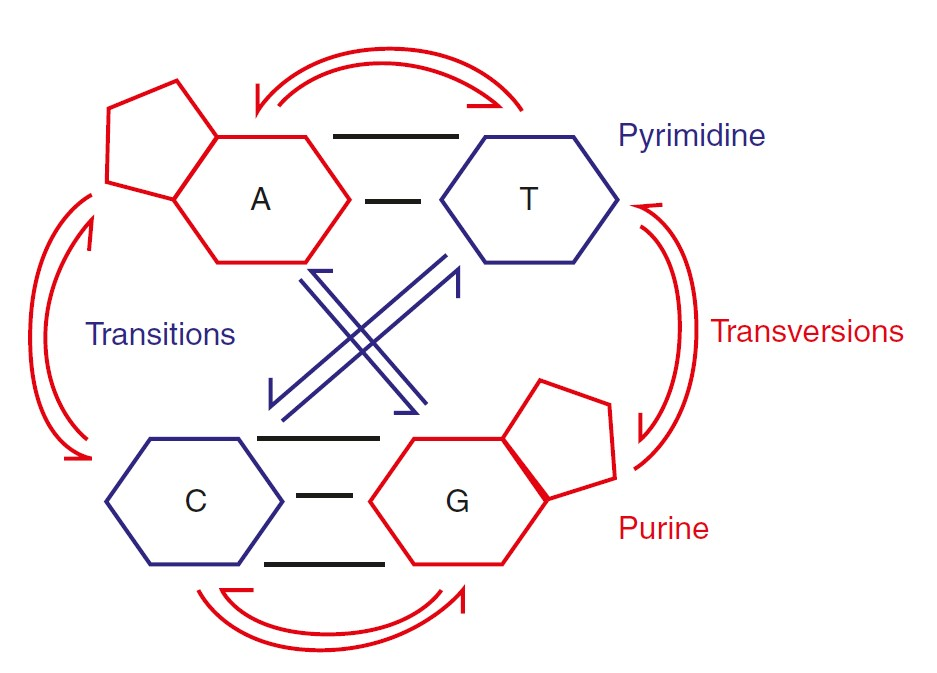
\includegraphics[width=0.5\textwidth]{Imagens/pointsmutatuins.jpg}
			}%
			\caption{Mutações Pontuais em único nucleotídio}
			\label{fig:mutacoesPontuais1}
		\end{figure}
		
		As \textcolor{CarnationPink}{Mutações em regiões de codificação} que são classificadas como mutações silent, missense, ou nonsense. Mutações em regiões não codificantes podem afetar a expressão e o splicing das regiões codificantes, mas não são tão fáceis de descrever. A \ref{fig:mutacoesPontuais2} mostra as possíveis mutações nas regiões de codificação, de modo que elas podem ser classificadas de acordo com a proteína (produto genético). 

		\begin{figure}[h]
			\centering
			\fcolorbox{DarkTurquoise}{white}{%
				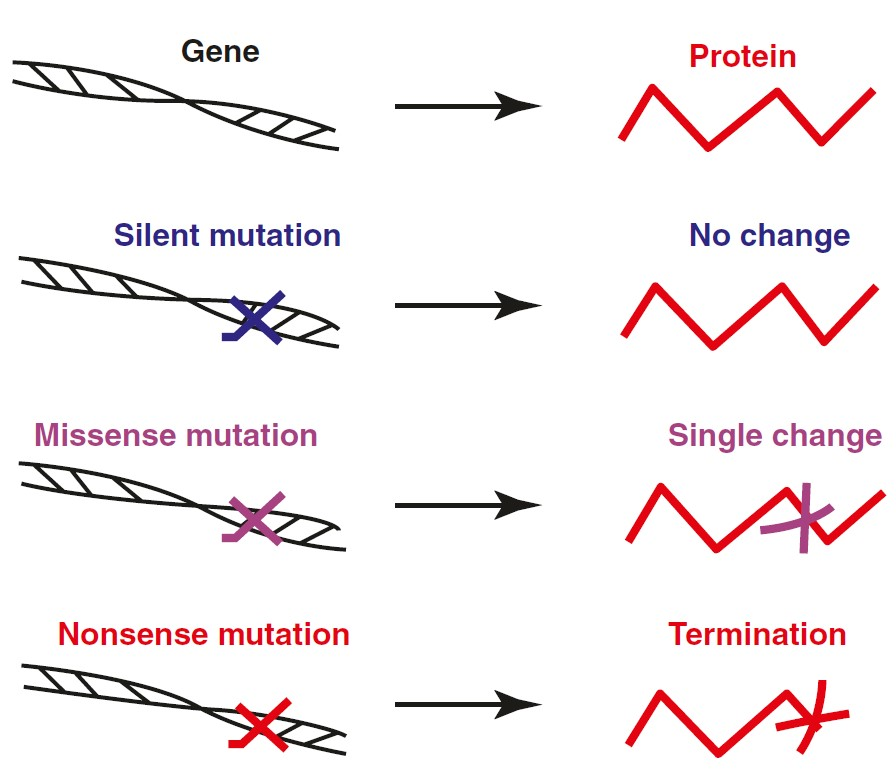
\includegraphics[width=0.5\textwidth]{Imagens/pointsmutatuins2.jpg}
			}%
			\caption{Mutações na região de codificação}
			\label{fig:mutacoesPontuais2}
		\end{figure}

		\textcolor{CarnationPink}{Pequenas inserções e deleções}, ocorridas em poucos pares de base, também são consideradas como mutações pontuais, onde estas mutações ocorrem quando a replicação do DNA “gagueja” e pula ou repete uma sequência. 

		As \textcolor{CarnationPink}{Mutações Cromossômicas}, também chamadas de mutações grosseiras, são grandes o suficiente de modo que afetam toda a estrutura do cromossomo, tendo como tamanho milhões de pares de base de extensão.  As \textcolor{MediumOrchid}{Deleções Grosseiras} ocorrem quando partes do DNA se desprendem do cromossomo e são permanentemente perdidas;  As \textcolor{MediumOrchid}{Translocações} ocorrem quando sequências quebradas de DNA são re-anexadas ao cromossomo errado.  As \textcolor{MediumOrchid}{Amplificações} ocorrem quando uma sequência de DNA é replicada várias vezes no mesmo ciclo celular.

	
		A \textcolor{CarnationPink}{Aneuploidia} é a perda ou o ganho de cromossomos inteiros. A célula humana normal possui dois pares de cromossomos 1 - 22 e dois cromossomos sexuais X  X(feminino) e X Y (masculino), ou seja, 46XX ou 46XY, de modo que qualquer coisa diferente disto é classificado como aneuploidia, exceto se tratando de células germinativas. A Aneuploidia ocorre quando os cromossomos não conseguem de dividir adequadamente durante a mitose. Nesses casos a maioria das células morrem através de um processo chamado catástrofe mitótica. Porém, algumas células conseguem sobreviver mesmo não se dividindo adequadamente, e portanto tornam-se células aneuploides, que podem ser classificadas como:

			\begin{enumerate}
				\item \textcolor{DarkTurquoise}{\textbf{Hipodiploidia:}} quando há menos de 46 cromossomos.
				\item \textcolor{DarkTurquoise}{\textbf{Hiperdiploidia:}}  quando há mais de 46 cromossomos.
				\item \textcolor{DarkTurquoise}{\textbf{Tetraploidia:}} quando existe exatamente o dobro do número normal de cromossomos (92 cromossomos). Isso acontece após o mecanismo de fusão celular.
			\end{enumerate}

	\section{Perda da Heterozigosidade}

		O heterozigoto se refere a um organismo que possui dois alelos diferentes para um determinado gene em um par de cromossomos homólogos. Cada alelo representa uma versão diferente do gene, que pode resultar em características diferentes.

		Os alelos podem ser classificados em dominantes e recessivos. O alelo dominante é expresso quando presente em apenas uma cópia, enquanto o alelo recessivo é expresso apenas quando presente em duas cópias. Portanto, em um heterozigoto, o alelo dominante será expresso, enquanto o alelo recessivo ficará mascarado.

		Por exemplo, no caso do gene para cor dos olhos em humanos, o alelo para olhos castanhos é dominante (B), e o alelo para olhos azuis é recessivo (b). Um indivíduo heterozigoto para esse gene teria a combinação Bb, o que resultaria na expressão da cor castanha dos olhos.
	
		Os seres humanos tem duas cópias de cada cromossomo e, portanto duas cópias de cada gene. Isso fornece proteção contra mutações recessivas. Mesmo com uma cópia mutada, a cópia saudável de um gene pode assumir sua função. A \textcolor{CarnationPink}{\textbf{perda de heterozigosidade (LoH)}} é usada para descrever qualquer locus gênico que esteja mutado e/ou perdido em ambos os cromossomos. Este é um mecanismo de mutação de “dois golpes”. Um cromossomo está com defeito há muito tempo (possivelmente herdado), enquanto o outro cromossomo foi deletado recentemente. A \ref{fig:perdaDaHeterozigosidade} mostra a perda de heterozigosidade que ocorre quando um gene é não-funcional em ambos os cromossomos, materno e paterno.

			\begin{figure}[h]
				\centering
				\fcolorbox{DarkTurquoise}{white}{%
					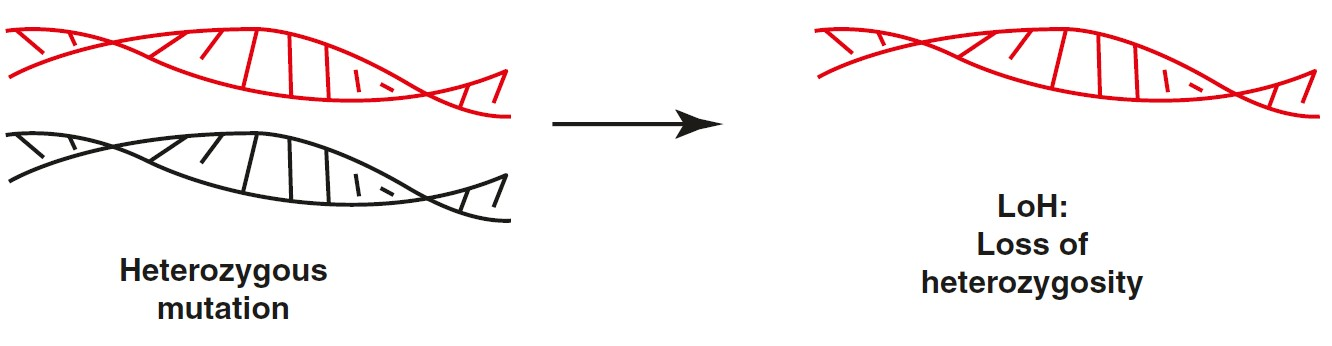
\includegraphics[width=0.5\textwidth]{Imagens/Lossofheterozygosity.jpg}
				}%
				\caption{Perda da Heterozigosidade}
				\label{fig:perdaDaHeterozigosidade}
			\end{figure}

	\section{Expressão Genética}
	
		Embora todas as células do corpo de uma pessoa possuam o mesmo genoma, as células de diferentes tecidos atuam de forma diferente. Isto é possível, sem alterar o genoma, através dos mecanismos de aumento e diminuição da expressão genética.

		Os tecidos possuem o mesmo genoma, o conjunto completo de genes presentes em uma célula ou organismo, mas desenvolvem funções diferentes devido a um processo chamado de diferenciação celular. Durante o desenvolvimento de um organismo multicelular, as células passam por um programa complexo de regulação genética que determina seu destino e função.

		As células-tronco são células indiferenciadas que têm o potencial de se transformar em diferentes tipos de células especializadas. À medida que um organismo se desenvolve, as células-tronco sofrem processos de divisão celular e diferenciação. Elas recebem sinais bioquímicos do ambiente interno e externo, como fatores de crescimento e interações com outras células, que ativam ou desativam determinados genes em seu genoma.

		Essa ativação ou desativação seletiva de genes é chamada de regulação gênica. Diferentes combinações de genes são ativadas em diferentes tipos de células, o que leva à produção de proteínas específicas e, por sua vez, a funções e características celulares distintas. Por exemplo, as células musculares ativam genes relacionados à contração muscular, enquanto as células do fígado ativam genes envolvidos no metabolismo de toxinas.

		A regulação gênica é um processo altamente complexo e é influenciada por diversos fatores, incluindo sinais químicos e físicos do ambiente celular, interações com outras células e estruturas tridimensionais do DNA. Esses fatores determinam quais genes serão ativados ou desativados em uma célula específica, permitindo que ela desenvolva uma função especializada.

		No aumento da expressão genética há fatores de transição positivos onde proteínas sinalizadoras podem se ligar diretamente ao DNA para induzir ou suprimir a transcrição, ocorrendo então a acetilação\footnote{A \textcolor{MediumOrchid}{\textit{acetilação}} é um processo caracterizado pela adição de um grupo acetila a resíduos de lisina em proteínas, geralmente catalisada por enzimas chamadas acetiltransferases. A acetilação está envolvida na regulação da atividade das proteínas, afetando a interação proteína-proteína e a estrutura das cromatinas, por exemplo.} da cromatina, onde abre-se a cromatina e induz a expressão genética.

		Na diminuição genética há a ação de fatores de transcrição negativos, chamados de repressores, que induzem a metilação\footnote{A \textcolor{MediumOrchid}{\textit{metilação}} é um processo caracterizado pela adição de um grupo metila a resíduos de aminoácidos, como lisina ou arginina. A metilação está envolvida na regulação da expressão gênica, estabilidade das proteínas e interações proteína-proteína.} da cromatina onde a cromatina se fecha e previne a expressão genética. 

		A \ref{fig:cromatinaExpressaoGenetiva} apresenta os possíveis estados da cromatina e sua relação com a expressão genética. A cromatina pode existir em um estado fechado (inativa) ou em um estado aberto (ativa). Seus estados são regulados pela acetilação ou pela metilação.


		\begin{figure}[h]
			\centering
			\fcolorbox{DarkTurquoise}{white}{%
				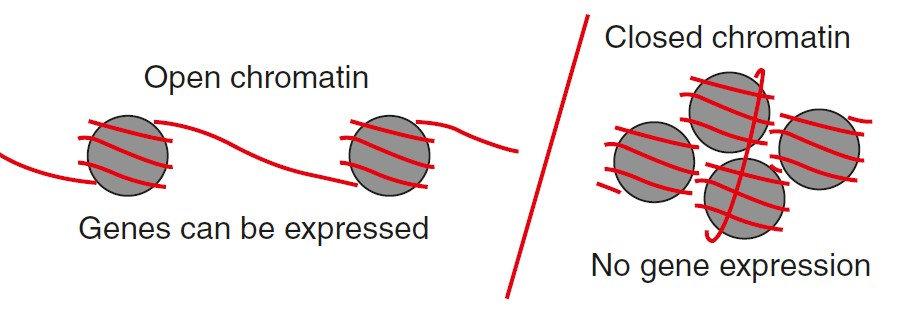
\includegraphics[width=0.5\textwidth]{Imagens/Chromatin may Closed chromatin.jpg}
			}%
			\caption{Cromatina na Expressão genética}
			\label{fig:cromatinaExpressaoGenetiva}
		\end{figure}

		Muitos genes humanos possuem múltiplas variantes de splicing de modo que um gene pode produzir diferentes produtos gênicos, através de um método chamado de Modificação da transcrição mRNA, que também permite uma diferente expressão genética para o mesmo genoma.

		A superexpressão e o silenciamento descrevem um aumento ou diminuição geral na expressão gênica. Esses termos incluem mutação (amplificação ou deleção do gene) e alterações epigenéticas.

		A regulação microRNA refere-se ao processo pelo qual pequenas moléculas de RNA, chamadas de microRNAs (miRNAs), desempenham um papel na regulação da expressão gênica em nível pós-transcricional. Os miRNAs são moléculas de RNA não codificantes, com cerca de 20-25 nucleotídeos de comprimento, que estão envolvidas em uma variedade de processos biológicos, incluindo o controle da expressão gênica. Na regulação microRNA (miRNA) dos níveis de mRNA e tradução de proteínas, as células sintetizam e usam pequenos miRNAs endógenos não codificantes para alterar os níveis de mRNA pós-transcricionalmente e, portanto, também os níveis de tradução de proteínas. Os níveis de miRNA são alterados em muitos tipos de câncer por amplificações, deleções e má regulação transcricional.

		Quando o miRNA se liga ao mRNA, ele pode ter diferentes efeitos, dependendo do grau de complementaridade e do contexto celular. Alguns dos principais mecanismos de regulação incluem:

		\begin{itemize}
			\item Inibição da tradução: o miRNA pode se ligar ao mRNA alvo de forma parcialmente complementar, impedindo a tradução do mRNA em proteína. Isso ocorre através da formação de um complexo ribonucleoproteico (RNP) que bloqueia o acesso dos ribossomos ao mRNA, inibindo assim a síntese proteica.
			\item Degradação do mRNA: em alguns casos, quando há uma complementaridade mais extensa entre o miRNA e o mRNA alvo, a ligação pode desencadear a degradação do mRNA. Isso resulta na redução da quantidade de mRNA disponível para sua tradução em proteína.
		\end{itemize}

		Por exemplo, descobriu-se que miR-15a e miR-16-1 são deletados em leucemias linfocíticas de células B, e miR-143 e miR-145 são deletados em câncer de pulmão e são considerados supressores de tumor. 
		
		Por outro lado, o cluster miR-17-92 que codifica vários miRNAs individuais é superexpresso em vários linfomas e em cânceres de pulmão, cólon e fígado, e é considerado oncogênico.
		
		A radiação pode alterar os níveis de miRNA e, dependendo do tipo de célula e da dose de radiação, os níveis podem ser induzidos ou reprimidos. O receptor EGFR e PI3K/AKT\footnote{Os receptores AKT são proteínas localizadas na membrana celular que ativam a via de sinalização do AKT quando são ativados por moléculas específicas chamadas ligantes. } é uma via pró-sobrevivência envolvida na resposta à radiação e é regulada por vários miRNAs, como o cluster miR-302-367 e miR-7. PTEN, um AKT\footnote{AKT, também conhecido como proteína quinase B (PKB), é um tipo de proteína quinase serina/treonina e está envolvido em várias vias de sinalização que regulam o crescimento, sobrevivência celular, proliferação e metabolismo.} negativo regulador, é regulado pelo miR-21.

	\section{Modificação Pós-Traducional}

		Após a tradução ocorre um processo de dobramento da cadeia de aminoácidos recém-sintetizada durante a síntese proteica. Após a tradução do RNA mensageiro (mRNA) em uma sequência de aminoácidos, a proteína precisa assumir uma estrutura tridimensional específica para desempenhar sua função corretamente.

		O dobramento correto da proteína é essencial para que ela adquira a estrutura tridimensional adequada, que é fundamental para sua função biológica. As proteínas são compostas por longas cadeias de aminoácidos, e a sequência específica desses aminoácidos determina a estrutura final da proteína. Durante o processo de dobramento, a cadeia de aminoácidos assume uma conformação espacial precisa, na qual as regiões hidrofóbicas (não tem afinidade com a água)  e hidrofílicas (tem afinidade com a água) da proteína se organizam de maneira apropriada.
		
		O dobramento incorreto, também conhecido como "dobramento impróprio" ou "misfolding", pode ocorrer devido a mutações genéticas, condições ambientais adversas ou fatores de estresse celular. Quando uma proteína não dobra corretamente, pode perder sua estrutura funcional e não ser capaz de desempenhar sua função normal. Em alguns casos, proteínas mal dobradas podem formar agregados ou se tornarem tóxicas para a célula, contribuindo para doenças como Alzheimer, Parkinson e outras doenças neurodegenerativas.

		A modificação pós-traducional é um processo que ocorre após a síntese de uma proteína durante a tradução do RNA mensageiro (mRNA) em uma sequência de aminoácidos. É um mecanismo importante para a diversidade e regulação das proteínas, uma vez que a estrutura e função de uma proteína podem ser alteradas através dessas modificações.

		Uma vez que um gene produziu uma proteína que se dobrou adequadamente após a tradução, a função e a atividade de uma proteína são frequentemente reguladas por outros processos/modificações dentro da célula.

		Em outras palavras, após a síntese da proteína a partir do gene, a função e a atividade dessa proteína podem ser controladas e reguladas por outros processos ou modificações que ocorrem dentro da célula. Embora o gene forneça as instruções para a produção da proteína, outras etapas e mecanismos dentro da célula podem influenciar e modificar como a proteína funciona e interage com outros componentes celulares. Isso destaca a complexidade da regulação das proteínas e como múltiplos processos estão envolvidos na determinação de suas funções específicas.

		Os mecanismos relacionados à \textcolor{CarnationPink}{\textbf{modificação da proteína}} são: \textbf{Fosforilação/desfosforilação, Hidroxilação, Dimerização e Crosslinking(Reticulação)}. Ja o processo relacionados à \textcolor{CarnationPink}{\textbf{modificação do tempo de vida da proteína}} é chamado de \textbf{Ubiquitinação}. A proteína pode ser mudada de local através de um processo chamado de \textbf{Translocação}.
		
		As reações de textcolor{CarnationPink}{\textbf{Fosforilação e Desfosforilação}}, são os principais mecanismos de modificação da função da proteína, uma vez que os grupos de fosfatos são os grupos químicos de alta energia mais comuns na célula. Na fosforilação ocorre a adição de um grupo fosfato a resíduos de aminoácidos específicos, como serina, treonina ou tirosina, por meio de enzimas chamadas quinases, enquanto que a desfosforilação é mediada pelas enzimas fosforilases que removem o grupo fosfato desses aminoácidos.

		As quinases e fosforilases são classificadas pelo aminoácido sobre o qual são capazes de atuar: As \textcolor{DarkTurquoise}{Tirosina quinases (TKs)}  incluem todos os receptores de fator de crescimento, como por exemplo as enzimas EGFR, Her2/Neu, PDGFR, VEGFR e IGFR; Exemplos de \textcolor{DarkTurquoise}{Serina/treonina quinases} são MAPK, ERK e TGF$\beta$R.

		A \textcolor{CarnationPink}{\textbf{Hidroxilação}} refere-se à adição de grupos hidroxila (-OH) a resíduos específicos de aminoácidos presentes na cadeia polipeptídica da proteína. Essa modificação pós-traducional pode ocorrer em diversos aminoácidos, sendo a prolina e a lisina os mais comumente hidroxilados.

		A \textcolor{CarnationPink}{\textbf{Dimerização}} refere-se à formação de um complexo constituído por duas subunidades idênticas ou diferentes de uma determinada proteína e pode ocorrer de diferentes maneiras sendo influenciada por várias interações, incluindo ligações hidrofóbicas, ligações de hidrogênio, interações eletrostáticas e interações van der Waals entre as subunidades proteicas, o que leva a várias implicações funcionais para as proteínas envolvidas.

		A \textcolor{CarnationPink}{\textbf{Reticulação}} refere-se à formação de ligações covalentes entre duas ou mais moléculas de proteínas, resultando na ligação cruzada entre elas. Essas ligações covalentes podem ocorrer entre resíduos de aminoácidos específicos, como cisteínas, lisinas ou tirosinas, dentro das cadeias polipeptídicas das proteínas. 

		A \textcolor{CarnationPink}{\textbf{Ubiquitinação}} é um processo em que uma pequena proteína chamada ubiquitina é ligada covalentemente a uma proteína-alvo. A ligação da ubiquitina ocorre por meio de uma série de reações enzimáticas, envolvendo enzimas conhecidas como ligases de ubiquitina. A ubiquitina pode ser adicionada a uma única proteína (monoubiquitinação) ou formar cadeias de ubiquitina (poliubiquitinação) ligadas à proteína-alvo. 

		A \textcolor{CarnationPink}{\textbf{Translocação}} refere-se ao movimento de uma proteína de um compartimento celular para outro. Esse processo pode ocorrer através das membranas celulares, envolvendo a passagem da proteína por meio de poros ou canais, ou pode envolver o transporte dentro do retículo endoplasmático, complexo de Golgi ou outras organelas membranosas.

	\section{Sinalização Molecular: Receptores e Ligantes}

		Os receptores e os ligantes são componentes essenciais na comunicação e sinalização celular. Os receptores são proteínas localizadas na superfície das células ou no interior delas, e eles têm a capacidade de reconhecer e se ligar a moléculas específicas chamadas de ligantes.

		Os ligantes podem ser moléculas pequenas, como hormônios, neurotransmissores, neurotransmissores, íons ou compostos químicos, ou mesmo macromoléculas, como proteínas ou fragmentos de proteínas. Esses ligantes têm afinidade e especificidade pelos receptores correspondentes, o que significa que eles se encaixam em sítios específicos nos receptores, semelhante a uma chave que se encaixa em uma fechadura.
	
		Quando um ligante se liga ao seu receptor, isso desencadeia uma série de eventos dentro da célula, resultando em uma resposta biológica específica. Essa resposta pode envolver a ativação de vias de sinalização intracelular, modulação da expressão gênica, alteração da atividade enzimática, regulação do fluxo iônico ou até mesmo a comunicação intercelular.

		Existem diferentes tipos de receptores e ligantes, e sua interação é altamente específica. Alguns exemplos comuns incluem receptores de hormônios, como os receptores de insulina, receptores de neurotransmissores, como os receptores de dopamina, e receptores de fatores de crescimento, como os receptores de fator de crescimento epidérmico (EGFR).

	\section{Perfil de Expressão Gênica}

		O desenvolvimento de perfil de expressão gênica é uma técnica que permite analisar a atividade dos genes em um determinado tecido, célula ou organismo em um determinado momento. Essa técnica fornece informações sobre quais genes estão ativos (expressos) e em que níveis estão sendo expressos.

		Existem várias abordagens para a criação de perfil de expressão gênica, mas uma das técnicas mais comuns e amplamente utilizadas é a microarray de DNA ou RNA. Nesse método, pequenas sondas de DNA ou RNA complementares a sequências específicas de genes são fixadas em uma superfície sólida, formando uma matriz.
	
		A amostra de RNA mensageiro (mRNA) obtida do tecido ou célula de interesse é isolada e convertida em cDNA (DNA complementar). O cDNA é então marcado com corantes fluorescentes, como cianina (Cy3) e fluorocromo vermelho (Cy5), que permitem a detecção dos níveis de expressão dos genes.
	
		O cDNA marcado é hibridizado na matriz de microarray, onde ocorre a ligação específica entre as sondas de DNA fixadas e os cDNAs presentes na amostra. A intensidade da fluorescência resultante é capturada e quantificada para cada sonda, representando a expressão relativa do gene correspondente na amostra.
	
		Além da microarray, outras técnicas de perfil de expressão gênica incluem a tecnologia de sequenciamento de nova geração (NGS), como o RNA-Seq, que permite a análise abrangente do transcriptoma de uma amostra, identificando todos os transcritos presentes, incluindo genes expressos, isoformas alternativas e até mesmo novos genes.
	
		Essas técnicas fornecem uma visão detalhada da expressão gênica em diferentes condições, permitindo a identificação de genes diferencialmente expressos entre diferentes amostras ou grupos experimentais. Essa análise pode revelar informações importantes sobre a função dos genes, as vias de sinalização envolvidas e os mecanismos subjacentes a determinados processos biológicos ou condições patológicas.
	
		O perfil de expressão gênica é uma ferramenta amplamente utilizada em estudos de biologia molecular, genética, medicina e pesquisa biomédica em geral. Ela desempenha um papel fundamental na compreensão dos processos biológicos, no diagnóstico de doenças, na identificação de biomarcadores e no desenvolvimento de terapias personalizadas.

	\section{Tipos de Morte Celular}

		Existem diversos mecanismos de morte celular, dentre eles os principais são:

		\begin{itemize}
			\item \textcolor{DarkTurquoise}{\textbf{Apoptose:}}  é um tipo de morte celular programada que ocorre como parte normal do desenvolvimento e da homeostase celular.Neste mecanismo de morte celular envolve os seguintes processos:
			\begin{enumerate}
				\item Sinalização da apoptose: A apoptose pode ser desencadeada por diferentes estímulos, como sinais extracelulares, danos no DNA, estresse celular, falta de nutrientes ou fatores de crescimento, entre outros. Esses estímulos ativam vias de sinalização específicas que levam à indução da apoptose.
				\item Ativação de cascatas de caspases: A caspase é uma família de enzimas proteolíticas chave na apoptose. A ativação das caspases é um passo crítico no processo apoptótico. Existem duas vias principais de ativação de caspases na apoptose: a via intrínseca (mitocondrial) e a via extrínseca (receptor-dependente). Ambas as vias levam à ativação de caspases executoras, que são responsáveis pela degradação de proteínas celulares essenciais para a sobrevivência da célula.
				\item Alterações morfológicas: Durante a apoptose, a célula passa por várias alterações morfológicas características. A célula encolhe e se condensa, formando corpos apoptóticos. A membrana celular também sofre alterações, como exposição de fosfatidilserina na superfície externa, o que sinaliza a células vizinhas ou células fagocíticas para a remoção dos restos celulares.
				\item Fragmentação do DNA: A fragmentação do DNA é uma característica distintiva da apoptose. O DNA nuclear é fragmentado em fragmentos de tamanho característico, conhecidos como "fragmentação do DNA em ladder", que podem ser detectados por técnicas como eletroforese em gel de agarose.
				\item Fagocitose e eliminação: Os corpos apoptóticos e outros resíduos celulares resultantes da apoptose são reconhecidos e englobados por células fagocíticas, como macrófagos, para serem eliminados de forma segura do tecido.
			\end{enumerate}

				É importante ressaltar que a apoptose é um processo altamente regulado, evitando a liberação de conteúdo celular que poderia causar danos e inflamação ao tecido circundante. Além disso, a apoptose também desempenha um papel na manutenção do equilíbrio entre proliferação celular e morte celular, essencial para a homeostase adequada nos tecidos e órgãos.

				A regulação da apoptose envolve uma complexa rede de sinalização, que inclui proteínas pró-apoptóticas e antiapoptóticas, além de diversas vias de sinalização intracelular. Disfunções na regulação da apoptose podem estar associadas a doenças, como câncer, doenças neurodegenerativas e doenças autoimunes.

			\item \textcolor{DarkTurquoise}{\textbf{Necrose:}} A necrose é um tipo de morte celular não programada que ocorre em resposta a estresses extremos, como lesões físicas, privação de oxigênio, infecções ou exposição a substâncias tóxicas. A necrose é caracterizada pela ruptura da membrana celular, liberação de conteúdo celular e resposta inflamatória. Ao contrário da apoptose, a necrose não é uma forma controlada de morte celular.
			
				Os principais eventos em uma morte celular via necrose são:

				\begin{enumerate}
					\item Danos celulares extensos: A necrose ocorre em resposta a danos celulares severos que excedem a capacidade de reparo da célula. Isso pode ser causado por diferentes fatores, como trauma físico, falta de oxigênio (isquemia), exposição a toxinas ou infecções graves.

					\item Inchaço celular e ruptura da membrana: Como resultado dos danos, a célula sofre inchaço e perda de controle da homeostase osmótica. Isso leva à ruptura da membrana plasmática, resultando em liberação de conteúdo celular para o ambiente extracelular.
					
					\item Inflamação: A morte celular por necrose é frequentemente acompanhada por uma resposta inflamatória. A liberação de conteúdo celular, incluindo enzimas e moléculas sinalizadoras, desencadeia uma resposta imunológica que envolve a ativação de células inflamatórias, como macrófagos, e a liberação de mediadores inflamatórios.
					
					\item Dano ao tecido circundante: Ao contrário da apoptose, que resulta na remoção controlada e sem danos das células, a necrose pode causar danos ao tecido circundante devido à liberação de enzimas e substâncias tóxicas das células danificadas.
					
					\item Processos secundários: A morte celular por necrose pode desencadear outros processos secundários, como reações oxidativas, liberação de citocinas inflamatórias, ativação de vias de estresse celular e resposta imune.
				\end{enumerate}

			\item \textcolor{DarkTurquoise}{\textbf{Autofagia:}} A morte celular por autofagia, também conhecida como autofagia mediada pela morte (autophagy-dependent cell death), é um processo pelo qual as células morrem como resultado de uma autofagia excessiva ou defeituosa. A autofagia é um mecanismo celular de degradação e reciclagem de componentes celulares, incluindo organelas danificadas ou envelhecidas, proteínas malformadas e agregados intracelulares. Quando a autofagia é ativada em níveis excessivos ou prolongados, pode levar à morte celular.
			\item \textcolor{DarkTurquoise}{\textbf{Catástrofe Mitótica:}} é um tipo de morte celular que ocorre devido a falhas graves no processo de divisão celular, chamado mitose. Durante a mitose, as células se dividem em duas células filhas idênticas, cada uma com o mesmo conjunto de cromossomos.

			Quando ocorrem erros críticos durante a mitose, como danos no DNA, erros na segregação dos cromossomos ou danos no aparato mitótico, a célula pode entrar em um estado de catástrofe mitótica. Nesse estado, a célula não consegue completar a divisão celular normalmente e acaba morrendo.
			
			A morte celular por catástrofe mitótica pode ocorrer de diferentes maneiras:
			\begin{enumerate}
				\item Formação de multipolaridade: Durante a mitose, os cromossomos normalmente se alinham em uma placa equatorial e são segregados de forma precisa para as células filhas. No entanto, em condições de catástrofe mitótica, podem ocorrer erros na formação do fuso mitótico, resultando em uma distribuição anormal dos cromossomos em múltiplos polos. Isso leva a uma segregação cromossômica desordenada e à formação de células aneuploides (com número anormal de cromossomos), o que pode levar à morte celular.
				\item Atraso ou parada da mitose: Em algumas situações de catástrofe mitótica, ocorre um atraso ou uma parada no progresso da mitose. Isso pode ocorrer devido a danos no DNA, ativação de sinalização de resposta ao estresse ou outros defeitos no aparato mitótico. A célula fica presa em uma fase específica da mitose, incapaz de completar a divisão celular normalmente. Essa interrupção prolongada da mitose pode levar à ativação de vias de morte celular e, eventualmente, à morte da célula.
				\item Indução de morte celular programada: A catástrofe mitótica também pode levar à ativação de mecanismos de morte celular programada, como a apoptose. Os erros na segregação cromossômica e a ativação de sinalização de estresse podem levar à ativação de cascatas de morte celular, resultando em apoptose da célula.
			\end{enumerate}
			
			A catástrofe mitótica é frequentemente associada a condições de estresse celular, como danos no DNA, tratamentos com agentes quimioterápicos ou radioterapia, ou a presença de genes mutantes ou anormalidades genéticas. A morte celular por catástrofe mitótica é considerada um mecanismo de proteção do organismo, impedindo a proliferação de células danificadas ou geneticamente instáveis.
			
			No entanto, é importante destacar que nem todas as células que passam por catástrofe mitótica necessariamente morrem. Algumas células podem sobreviver, mas com alterações genéticas significativas que podem contribuir para o desenvolvimento de doenças, como câncer.
		\end{itemize}

	\section{Sinais Moleculares Radio-Induzidos}

		A exposição à radiação ionizante, pode causar uma variedade de danos nas células e tecidos do organismo. Esses danos podem desencadear uma série de sinais moleculares que são característicos da resposta celular à radiação de modo que as células podem responder à radiação de diferentes maneiras. Dentre os sinais radio-induzidos podemos destacar:

		\begin{itemize}
			\item Quebra do DNA: A radiação ionizante pode causar quebras nas moléculas de DNA, incluindo quebras de cadeia simples e dupla. Essas quebras podem ocorrer diretamente no DNA ou através da geração de espécies reativas de oxigênio, que danificam o DNA. A detecção de danos no DNA através das proteínas ATM ATR é um dos principais sinais moleculares que desencadeiam a resposta celular à radiação.
			
			\item Parada do Ciclo Celular: A radiação ionizante pode induzir a parada do ciclo celular em diferentes pontos, dependendo da dose e do tipo de radiação envolvido, podendo ser devido ao Dano direto no DNA, Ativação da resposta ao dano ao DNA, Danos nos centrossomos\dots

			\item Ativação de vias de reparo do DNA: Em resposta aos danos no DNA, as células ativam vias de reparo do DNA para corrigir os danos e manter a integridade genômica. Isso inclui vias como reparo por excisão de nucleotídeos (NER), reparo por recombinação homóloga (HR), reparo por junção de extremidades não homólogas (NHEJ), entre outras.
			
			\item Ativação de vias de sinalização celular: A radiação ionizante pode ativar várias vias de sinalização celular, como a via do fator de transcrição p53, que desempenha um papel central na resposta ao estresse celular e na regulação da morte celular programada (apoptose). A ativação de vias de sinalização celular desencadeia uma resposta adaptativa e de sobrevivência da célula.
			
			\item Estresse oxidativo: A radiação ionizante pode levar à geração de espécies reativas de oxigênio (ROS) dentro das células. O aumento do estresse oxidativo desencadeia uma cascata de eventos moleculares, resultando em danos oxidativos adicionais nas moléculas celulares, incluindo lipídios, proteínas e DNA.
			
			\item Inflamação: A exposição à radiação pode desencadear uma resposta inflamatória nos tecidos irradiados. Isso envolve a liberação de citocinas inflamatórias e a ativação de células imunes, como macrófagos e linfócitos, que podem contribuir para a resposta à radiação e os efeitos tardios da exposição.
			
			\item Fibrose: A fibrose radioinduzida é uma resposta cicatricial excessiva e desregulada do tecido conectivo, resultando na formação de tecido fibroso rígido e endurecido (semelhante a uma cicatriz). Esse processo pode ocorrer como uma complicação tardia da exposição à radiação, especialmente em áreas onde ocorreu o tratamento.
		\end{itemize}

	Um efeito agudo da radiação é o Dano ao DNA:

		\begin{enumerate}
			\item O Dano no DNA é detectado pelas proteínas ATM/ATR;
			\item Quando uma célula reconhece que está danificada, uma célula proficiente em reparo tentará reparar o dano. Ao mesmo tempo, deve decidir como reagirá a esse dano onde a célula pode decidir parar de crescer e até mesmo se matar (apoptose) se estiver muito danificada.
				\begin{itemize}
					\item Via p53: Uma proteína que é pró-reparo, pró-parada e pró-apoptose.
					\item Vias da ceramida: A ceramida é um lipídio que é pró-parada e pró-apoptose.
					\item As vias de “parada e morte” tendem a prevenir a malignidade, pois impedem a proliferação de células mutantes. No entanto a perda de células em tecidos normais pode levar à perda de função
				\end{itemize}
			\item A célula também pode decidir proliferar e sobreviver, compensando o dano crescendo mais rápido.
				\begin{itemize}
					\item Via Fos/jun/myc: Pró-crescimento e anti-apoptose.
					\item As vias de “sobrevivência e crescimento” podem predispor à malignidade, pois permitem que as células mutantes cresçam. No entanto eles também são responsáveis por repovoar os tecidos normais após uma lesão.
				\end{itemize}

		\end{enumerate}

	Efeitos tardios - Inflamação e Fibrose:

		\begin{enumerate}
			\item A inflamação é uma resposta normal à lesão e pode ajudar a combater a infecção. Este processo é caracterizado por:
				\begin{itemize}
					\item Aumento do fluxo sanguíneo;
					\item Resposta imunológica melhorada;
					\item Aumento da renovação celular: tanto a morte celular quanto a proliferação são aumentadas.
				\end{itemize}

			\item Mais tarde, ocorre a fibrose (endurecimento do tecido), caracterizado por:
				\begin{itemize}
					\item Aumento da produção de matriz extracelular semelhante a cicatriz;
				\end{itemize}
		\end{enumerate}

\bibliography{ref.bib}
\end{document}